\chapter{BB84: Single-photon QKD}

This chapter introduces single-photon QKD, and particularly the first single-photon QKD protocol known as BB84, named for Charles Bennett and Giles Brassard, who developed it in 1984.

\section{Three phases of cryptographically secure communication}

% So, Step One: what are the "Three Phases of Cryptographic Secure Communication"?

Secure communication using encryption proceeds roughly in the following three phases: first, the parties need to authenticate each other, meaning that they prove they really are who they say they are and not somebody else. Second, they have to select or generate a key that they will use for encoding their messages.  Third, after the key is generated, they encode their messages and encrypt their data, then send them to the other party where they will be decrypted -- the actual bulk data transfer phase of the conversation.

Authentication between Alice and Bob usually proceeds in the following way: first, Alice says, "I'm Alice," to Bob. Then Bob can say, "Okay, you're Alice, I'm Bob". But of course, anybody could send that reply, so Alice's question is: "Why should I believe you? Why should I trust that you are really the person that you're claiming to be?" And Bob, of course, has the same questions.

Generally, the procedure two parties use to authenticate each other depends on one of three things: something you \emph{are}, something you \emph{have}, or something you \emph{know}. (This applies as well in the real world; trying to get into a private club or a 1920s U.S. speakeasy might involve personal recognition, a physical token such as an actual key, or a password you have been given by someone else.)  In particular the last one is quite important, because you know that the party that you are trying to communicate knows something, for example a secret pre-shared between the two parties, or generally and flexibly the private key corresponding to a particular public key, and that can be used as an authentication device.

After authentication, Alice and Bob have to generate a \emph{cryptographic key} (or just "key"). There are many different ways to exchange keys, such as Diffie-Hellman key exchange, which we don't need to go into here. The key will be subsequently used for encrypting the message, but one problem with the key is that once it is generated, it cannot be used forever. It has to be changed at regular intervals in order to ensure that the encrypted data remains secure.

Once the key is generated, Alice encrypts her message with the key. She sends it to Bob, where he will use his share of the generated key to decrypt the message and read it.  Typically, this \emph{bulk data encryption} phase of the conversation uses a \emph{symmetric key cryptosystem}, where Alice and Bob use the same key to encrypt and decrypt the messages. Common forms include the now-outdated Data Encryption Standard (DES), the stronger (and still in use) 3-DES, and the modern Advanced Encryption Standard (AES). Less common is one-time pad (OTP)\index{one-time pad (OTP)}. Later we will describe the one-time pad, which is also known as the \emph{Vernam cipher}\index{Vernam cipher}.

Quantum key distribution, or QKD, is used in the second phase of this process.  Before we go into QKD, let's look briefly at how keys are established today when you use the Internet.

\section{Private vs. public key}

We have two parties, Alice and Bob, who are trying to communicate, and they can communicate over a public channel. "Public" means that anybody has access to this channel, so any message that they transmit can be heard and intercepted by any other party. So this channel is not secure, in the sense that anybody can read any message that Alice and Bob send. And yet, somehow Alice and Bob need to authenticate each other and prepare the key to be used for the bulk data encryption.

The simplest method is via a \emph{pre-shared key}. Alice and Bob meet somewhere, face to face, long before they want to communicate.  At this meeting, they create a shared secret between them, known to no one else.  This key can then be used later to authenticate each other, and to help generate the keys used for the bulk encryption.  Of course, for this method to work as a general mechanism for any two parties, every person must meet every other person.  That requires $O(N^2)$ meetings for $N$ people, which is obviously not practical.

To compensate for this shortcoming, instead we use mechanisms that don't require this prior agreement. One method is known as \emph{public key cryptography}\index{public key cryptography}. Alice generates two keys: one is known as the "public key" and the other one is known as the "private key".  They are a mathematically related pair.  In public key cryptography, the public key is used to encrypt the message, but it cannot be used to decrypt the message. 
The private key is needed to decrypt the message.  For this reason, public key cryptography is sometimes called \emph{asymmetric} cryptography.  Bob's public key is published in some fashion that allows Alice both to find Bob's key when she needs it, and trust that it is really Bob's key.  Alice uses that to encrypt her message, and then sends it to Bob. Bob then uses the private key (which he has kept secret) to decrypt Alice's message and read it.  The most prominent form of public key cryptography is known as RSA.

This process works, but it has some disadvantages. It is slow and computationally expensive. While it is theoretically possible for Alice to encrypt her actual message to Bob using public-key cryptography, which would combine the functions of authentication and encryption while eliminating the need for a separate key, it is not practical.  Therefore, we usually use three separate functions as described in the last section, with RSA for authentication, Diffie-Hellman for session key generation, and AES for bulk data encryption.

More important than the performance issues with public key cryptography, the security of both RSA and Diffie-Hellman is based on the idea that they are \emph{computationally secure}.  Of course, anybody listening to the channel is able to record the classical messages exchanged. In principle, an eavesdropper can break the encryption if they have access to a fast enough computer, either now (unlikely) or in the future (harder to guarantee)~\footnote{This is sometimes called "harvest now, decrypt later".}.  Therefore, RSA and Diffie-Hellman are not unconditionally secure~\footnote{Cryptographers are working to replace these mechanisms, in a broad push called \emph{post-quantum cryptography}, or PQC.  As of this writing, the first major phase of this process is nearing completion.}.

A crucial point is that quantum computers can in principle break some computationally secure protocols, notably RSA and Diffie-Hellman, with relative ease~\footnote{The details of this possibility are a very long discussion.}. So, how can we actually establish a secure connection between Alice and Bob? An alternative is to use some generator, some hypothetical device, that can generate a secret key, and that key is then shared with Alice and Bob in some secure fashion. Now, Alice and Bob are sharing some correlated secret key that only they know, and they can use it to encrypt their messages. For example, Bob encrypts a message, then sends it to Alice, who uses her knowledge of the secret key to decrypt it and read the message.

The bulk encryption mechanism can be AES, introduced in the last section, but the details are beyond the scope of this book. Or, we can encrypt one bit of message using one bit of key material.  One way to do this using an XOR operation.  If $m_i$ is the $i$th bit of the message, $k_i$ is the $i$th bit of the key, and $c_i$ is the $i$th bit of the ciphertext, or encrypted message, then $c_i = m_i \oplus k_i$.  This approach is known as \emph{one time pad}\index{one-time pad (OTP)} or the \emph{Vernam cipher}\index{Vernam cipher}, and it is provably secure. It cannot be broken, provided that the key material was generated in a secure and random fashion and, critically, is used only once. If Alice has a message of $n$ bits that she's trying to send to Bob, she requires a secret key that's at least $n$ bits long, and once she uses that key to encrypt her message she cannot use it again. If she has some other thing to say to Bob, they require a completely new and fresh secret key to ensure security. So, it's not very efficient in the sense that it requires a large number of key bits, at least as many as the message itself.

That's actually pretty good, but there is one remaining question if we want to use the one-time pad, and that's how we actually distribute this key.  Perhaps our hypothetical key generator is used only during Alice and Bob's face-to-face meeting.  But, we already know that that is impractical.  Our only alternative is to use the public channels available.  The classical public channel is subject to being recorded, as noted above, but a quantum channel, even if nominally public, offers unique properties that allow us to guarantee that no one is listening in.  We will see how this can be achieved in the next section.

\section{BB84 Protocol}
\label{sec:bb84-protocol}

BB84 is a quantum protocol.  Alice and Bob can utilize a public quantum channel, as well as their public classical channel.  Alice begins the protocol by generating two $n$-bit random strings. We're going to call the first $n$-bit string $a$.  We denote the bits $a_1$, $a_2$, up to $a_n$. The second bit string is $b$, with $b_1$, $b_2$, all the way up to $b_n$.  Then, Alice creates quantum states according to these bit strings.

Alice uses one bit from each string $a$ and $b$ to create one qubit. She creates $n$ such qubits, and the whole state will be denoted by \ket{\psi}. If her bits $a_k = 0$ and $b_k = 0$, then she encodes the qubit $\ket{\psi_{00}} = \ket{0}$.  For different values of $a_k$ and $b_k$, she will encode a different qubit state.  More completely, she uses the values $a_k$ to determine the encoded bit and $b_k$ to determine the encoding basis, giving the states
\begin{equation}
\begin{array}{ll}
\left|\psi_{00}\right\rangle=|0\rangle, & \left|\psi_{01}\right\rangle=|+\rangle \\
\left|\psi_{10}\right\rangle=|1\rangle, & \left|\psi_{11}\right\rangle=|-\rangle
\end{array}
\end{equation}
to make the complete qubit string
\begin{equation}
|\psi\rangle=\bigotimes_{k=1}^n\left|\psi_{a_k b_k}\right\rangle.
\end{equation}
We can see that the bit coming from the bit string $b$ determines the basis of Alice's encoding. If it's zero, she prepares the qubit in the $Z$ basis. If it's one, then she prepares the qubits in the $X$ basis. Then, $a_k$ chooses which state from the basis she prepares. If $a_k$ is zero, she prepares the $+1$ eigenstate, if it's one, she prepares the $-1$ eigenstate.

Notice that these states are not orthogonal. For example, if we take the inner product between \ket{\psi_{00}} and \ket{\psi_{01}}, we see that they are not orthogonal, meaning that their inner product is non-zero,
\begin{equation}
\left\langle\psi_{00} \mid \psi_{01}\right\rangle=\frac{1}{\sqrt{2}} \ne 0.
\end{equation}
In this particular case, the inner product is $1/\sqrt{2}$. It will be the same if we take, for example, 
$\braket{\psi_{10}}{\psi_{11}} = 1/\sqrt{2} \ne 0$. When the inner product is non-zero, it means that the two states are not perfectly distinguishable, and this is the crucial ingredient in this protocol. 

So what does it mean for two states to be non-distinguishable? Let's consider the case where we are measuring in the $Z$ basis, and we are given two states. Assume one state is \ket{0}, and the other state is \ket{1}. If this happens, we see that they are orthogonal, and we can perfectly distinguish them. So if we just keep measuring the incoming qubits, if the qubit is in \ket{0}, we will always get a $+1$ outcome. On the other hand, if the qubit is in \ket{1}, we will always get a $-1$ outcome. With certainty, we can distinguish whether the incoming qubit is a zero or a one.

The same thing applies if we are measuring in the $X$ basis, and we are given only \ket{+} or \ket{-}. If we keep measuring in $X$ and we are given the \ket{+} state, then the outcome will be always $+1$ with hundred percent probability. If on the other hand we are given the \ket{-} state, and we measured in the $X$ basis, we will get outcome $-1$ all the time. In this sense, we can distinguish plus and minus if we're measuring in the $X$ basis.

On the other hand, let's say that we are given the states \ket{0} or \ket{+}, and we measure in the $Z$ basis. So if we measure the \ket{0} state, as above we always get the $+1$ outcome, that's fine. But if we measure the second state, the \ket{+} state, there's a fifty percent probability that we get the outcome $+1$ and fifty percent probability that we get the outcome $-1$.

So, if we are given a state \ket{0}, all is good, but if we are given the state \ket{+}, sometimes we will get a $+1$ and sometimes we will get a $-1$. If our measurement result is $-1$, fine, we can say we know that this state is \ket{+}, but if we get the $+1$ outcome, we are unsure whether the state we were given was a \ket{+} or whether it was a \ket{0}. In this sense, the states are non-distinguishable. We can do the same thing in the $X$ basis, and here the scenario is reversed. With certainty, we can say that we get a $+1$ outcome if we were given a \ket{+}, but if we were given a \ket{0}, sometimes it will be a $+1$ and sometimes a $-1$.

Let's consider an example of the encoding, shown in Tab.~\ref{tab:bb84-example}. Let's say that Alice generates the two random strings $a = 01101$ and $b=11001$. She starts encoding.  First, she looks at the first bit in her string $b$, which is $1$, so she knows, "Now I have to encode in the $X$ basis," and the state that she prepares is a \ket{+} state because her first bit in the $a$ string is a $0$. So, that's her first qubit. To prepare the second qubit, she looks at the second bit in her string $b$, which is again $1$, so again she knows she has to prepare a state from the $X$ basis, and the state is given by the second bit in string $a$, which is $1$, therefore she prepares the state \ket{-}. Then she goes on until she prepares all $n$ qubits.

\begin{table}
\centering
\begin{tabular}{|c||c|c|c|c|c|}
\hline $i$ & 1 & 2 & 3 & 4 & 5 \\
\hline string $a$ & 0 & 1 & 1 & 0 & 1 \\
string $b$ & 1 & 1 & 0 & 0 & 1 \\
basis & $X$ & $X$ & $Z$ & $Z$ & $X$ \\
Encoded qubits & $|+\rangle$ & $|-\rangle$ & $|1\rangle$ & $|0\rangle$ & $|-\rangle$ \\
\hline
\end{tabular}
\caption[BB84 encoding example]{Alice encodes the qubits she sends, choosing a basis using a bit from $b$ and an eigenstate based on the corresponding bit from $a$.}
\label{tab:bb84-example}
\end{table}

Alice sends these qubits to Bob over the public quantum channel. Now, let's consider what Bob knows at this time. He actually doesn't know what these states are, because Alice did not share the secret string $b$ containing information about the preparation basis with anybody, she kept it secret. Therefore, all Bob knows is that he's receiving qubits and they can be any of the four possible states \ket{0}, \ket{1}, \ket{+} or \ket{-}. But, he goes on anyway and creates his own random bit string which we are going to denote as $b'$. Because he's expecting $n$ qubits, he generates $n$ bits: $\{b'_1, b'_2, \ldots\b'_n\}$.  He uses this bit string to pick the basis for measuring each of the qubits he receives.

Similarly to Alice, if the bit $b'_k$ is zero, then he measures in the $Z$ basis, and if it's in one then he measures in the $X$ basis. This allows him to generate his own random bit string which we will denote $a'$. If the outcome of the $k$th measurement on the qubits is $+1$, then he will assign $0$ to bit $a'_k$, if it's $-1$, then he assigns a bit $1$ to $a'_k$, and this way he generates his own $a'_k$ bit string, which will be random.

Next, Alice and Bob share some information with each other over a public classical channel. Alice shares her randomly generated bit string $b$, and Bob shares his randomly generated bit string $b'$.  This exchange shares information about the basis in which the qubits were prepared and in which they were measured.

If they measured and prepared in the same basis, they will keep the corresponding bits from $a$ and $a'$. If they measured in different bases, then they just discard the bits $a_k$ and $a'_k$. If Alice prepares in a certain basis and Bob measures in the same basis, the two possible states are orthogonal, meaning they are perfectly distinguishable by measurement in that basis, so it allows Bob and Alice to generate a perfectly correlated key. We denote the bits that they keep as $\bar{a}$ and $\bar{a'}$. These bits are perfectly correlated, meaning that these two shorter bit strings that they generated are equal. Now, they are sharing a key that they can use in the next step, which might be encryption of the data.

Let's look at an example, again considering a case where $n=5$, as shown in Tab.~\ref{tab:complete-bb84}. Alice has randomly generated two five-bit strings, $a$ and $b$. $b$ tells her in which basis she should encode, $a$ tells her what the state should be, so she prepares the following states: $\ket{-}\ket{0}\ket{+}\ket{-}\ket{1}$. Bob generates his own random $b'$ string. This bit string is different from Alice's $b$ because he doesn't know Alice's $b$ at this time. He measures in the basis given by $b'$.  You can see that in the first position Alice's preparation basis and Bob's measurement basis agree, so their classical bit $\bar{a_1}$ will agree.

% , so here the first bit in b-prime is one. Therefore, he measures in $X$ on the second bit. It's again one, therefore he measures in x, and so on and so forth. And you can see that since for the first qubit, Alice encoded the qubit in basis x, and Bob measured in basis x, therefore Bob will always, with hundred percent probability, get the outcome minus one, which we said corresponds to bit string a-prime which is equal to one. And we see that in this case, "a-prime one" is the same as Alice's "a one". 

On the other hand, for the second qubit, Alice prepared the qubit in the $Z$ basis, but because Bob's random bit $b'_2 = 1$, he measured in the $X$ basis.  With fifty percent probability he will obtain $0$, with fifty percent probability he will obtain $1$. They cannot be sure that they are really sharing a correlated bit, therefore they discard this bit. For the third qubit, $b_3 = b'_3$ and again Alice prepared in the same basis as Bob measured, therefore they know they can keep this bit and use it as part of their secret key. In this way, they are keeping a random subset of the bits, leaving a shorter string of key bits but all of which are one hundred percent correlated.  So, the shared key that they have is given by $\bar{a} = \bar{a'} = \{1, 0, 1\}$, as marked with the check marks in the table.


\begin{table}
\centering
\begin{tabular}{|c||c|c|c|c|c|}
\hline $i$ & 1 & 2 & 3 & 4 & 5 \\
\hline string $a$ & 1 & 0 & 0 & 1 & 1 \\
string $b$ & 1 & 0 & 1 & 1 & 0 \\
Alice's basis & $X$ & $Z$ & $X$ & $X$ & $Z$ \\
Encoded qubits & $|-\rangle$ & $|0\rangle$ & $|+\rangle$ & $|-\rangle$ & $|1\rangle$ \\
\hline string $b^{\prime}$ & 1 & 1 & 1 & 0 & 0 \\
Bob's basis & $X$ & $X$ & $X$ & $Z$ & $Z$ \\
string $a^{\prime}$ & 1 & $0 / 1$ & 0 & $0 / 1$ & 1 \\
\hline
use in $\bar{a}, \bar{a'}$ & \checkmark & & \checkmark & & \checkmark \\\hline
$\bar{a}, \bar{a'}$ & 1 & & 0 & & 1 \\\hline
\end{tabular}
\caption[A complete BB84 example for five bits.]{A complete BB84 example for five bits.  The check marks indicate bits where the selected preparation and measurement bases agree, giving a bit that can be used in the final agreed-upon key.}
\label{tab:complete-bb84}
\end{table}

\rdv{Replace this paragraph with a typeset algorithm (p.31 in slides, without eavesdropper detection; also doesn't have a separate step for exchange of bases)}
So, here's the summary of the protocol so far: Alice starts by generating two n-bit strings, a and b. "b" is used for basis of the preparation, whereas "a" tells which state of that particular basis Alice should prepare the qubit in. If b-k is equal to zero, then she prepares in the $Z$ basis, if b-k is equal to one, she prepares in the $X$ basis. Then, Alice sends these qubits to Bob over a public quantum channel. Bob measures randomly either in $Z$ or $X$ basis. After the measurements are completed, and only after that, they are allowed to share the information about the preparation basis and the measurement basis, and they keep the bits only where they prepared and measured in the same basis. Again, they do that because they are guaranteed that in this scenario, the results that are generated are hundred percent correlated. And whatever is left of the key, they use as a secret key for encoding and decoding their messages.

Now, so far, we have only considered the ideal scenario where there was no eavesdropper.  (In fact, we have not even checked for the presence of an eavesdropper yet.) Now let's say that somebody is listening to both the public classical channel and the public quantum channel. Next we are going to consider the effect of an eavesdropper whom we are going to name Eve, and see what effect she has on the protocol and how the protocol can actually discover the presence of such an eavesdropper.

\section{Eavesdropper detection}

In the previous section, we saw how the ideal protocol works. Now let's see what happens when we include the effect of an eavesdropper trying to gain access to the secret key that Alice and Bob are trying to generate.  We have the following scenario: Alice is communicating over a public quantum channel with Bob, and there is some third party Eve, that wants to intercept their messages.


\begin{figure}[H]
    \centering
    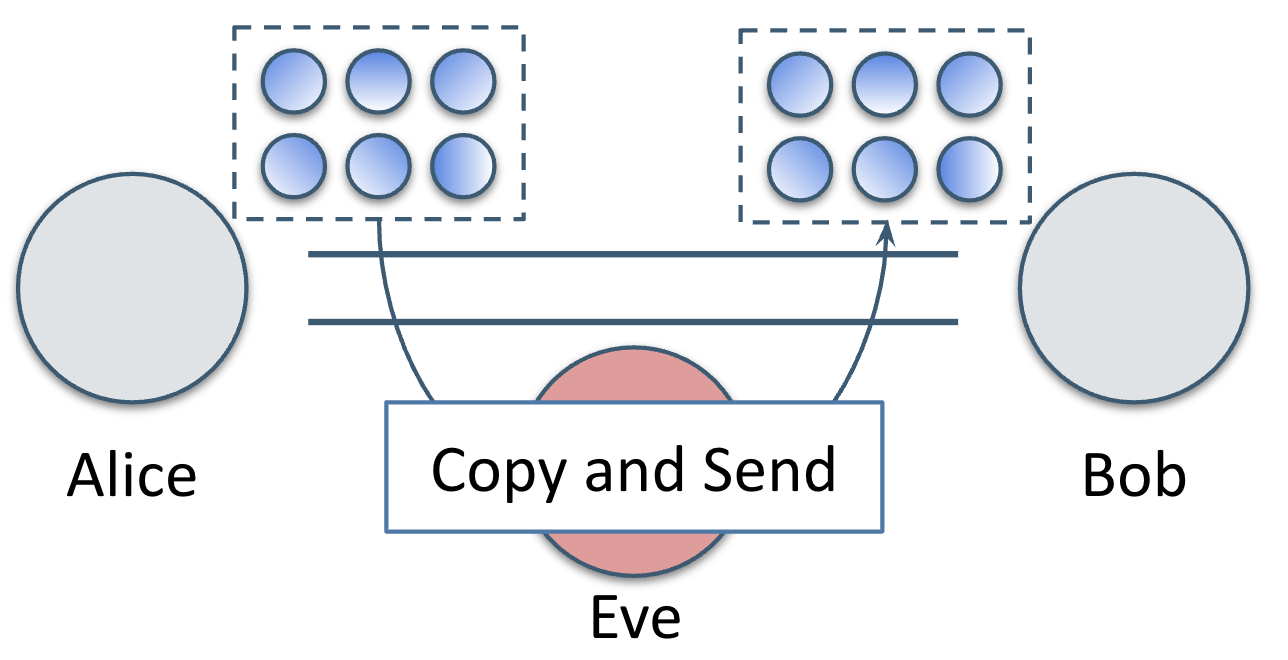
\includegraphics[width=0.8\textwidth]{lesson9/eve-copy-and-send.png}
        \caption[Eve's ideal (but impossible) eavesdropping arrangement]{Eve's ideal eavesdropping arrangement would be to copy the qubits sent by Alice, sending one copy to Bob and keeping the other copy for herself, but the no-cloning theorem makes that impossible.}
    \label{fig:eve-copy-and-send}
\end{figure}


So, what can Eve do? Let's imagine that she can intercept the qubits that Alice is sending over the public quantum channel, copy them and then resend them to Bob, as in Fig.~\ref{fig:eve-copy-and-send}. If she could do that, she could hold her copy of the qubits, wait until Alice announces her measurement bases, then measure her copy.  That would give her access to the protocol and the qubits, and also subsequently the secret quantum key. Luckily for us, it is physically impossible for Eve to do that due to the no-cloning theorem\index{no-cloning theorem} we saw in the previous chapter (Sec.~\ref{sec:8-3_no-cloning}).
%She cannot simply take them, make a copy of the qubit, and then resend the qubits to Bob.

If Eve cannot copy the qubits and hold them, then in order for Eve to gain any access to the information that Alice is trying to share with Bob, she has to measure the qubits. What can happen in this case? Eve has to guess the basis of measurement, because remember, the preparation basis stored in the bit string $b$ is still kept secret by Alice. That basis has not yet been communicated over a public classical channel to Bob. Without access to this information, Eve has to pick either the $X$ or $Z$ basis at random for her measurement, and may disturb the qubit.

\begin{figure}[H]
    \centering
    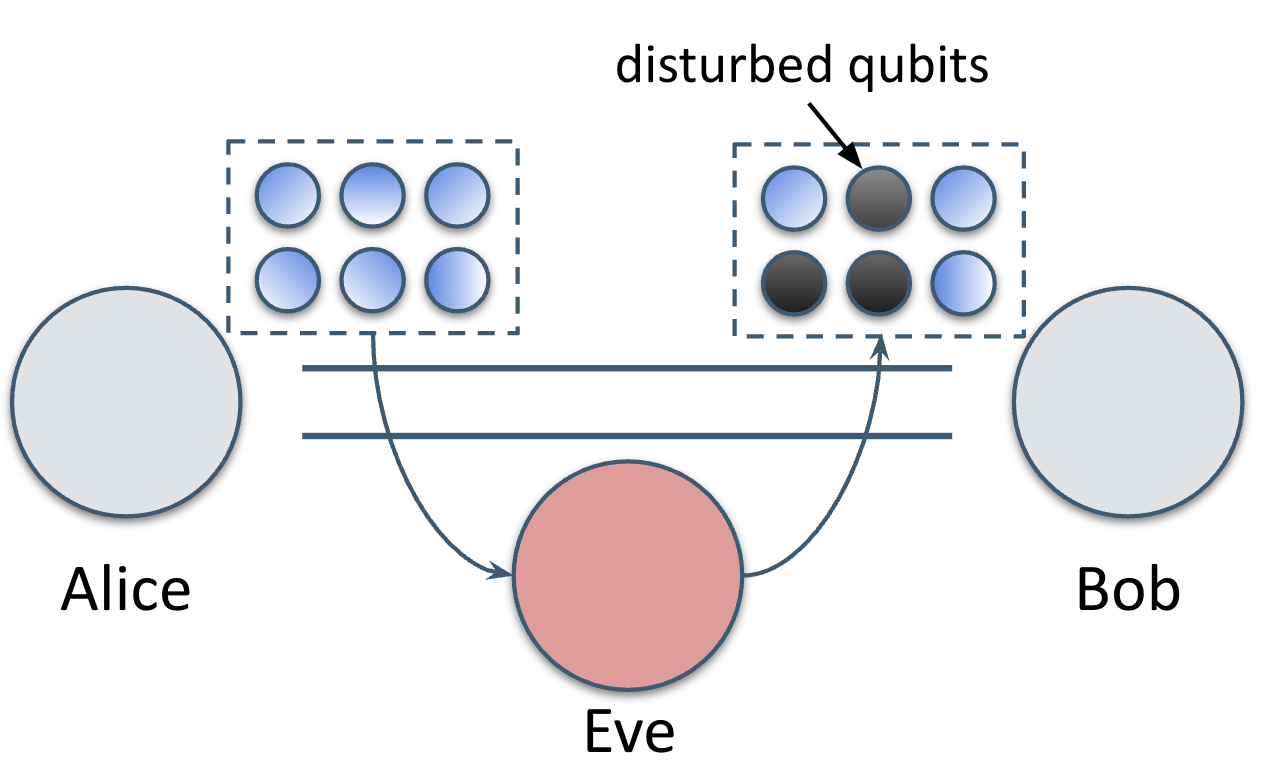
\includegraphics[width=0.8\textwidth]{lesson9/eve-disturbance.png}
        \caption[Eve's measurements disturb the qubits]{If Eve tries to measure  the qubits sent by Alice, then send them on to Bob, the disturbance she introduces will be easily detected.}
    \label{fig:eve-disturbance}
\end{figure}

For example, if Alice prepares the qubit in the $X$ basis, and Eve measures in the $X$ basis, then we have seen that in such a scenario, there is no disturbance. The qubit is still projected onto the same state that it was prepared in, leaving the state of the qubit unchanged. However, if Alice's preparation basis is $Z$ and Eve's measurement basis is $X$, things are different. The qubit originally prepared by Alice was either in \ket{0} or in \ket{1}.  But by measuring in the $X$ basis, Eve is now projecting the qubit onto the either the \ket{+} state or the \ket{-} state. She has disturbed the state, forcing it into an eigenstate of the wrong basis. Similarly, where Alice prepares in the $X$ basis and Eve measures in the $Z$ basis, the state will be projected into a different state than the one that was prepared. This is the main principle Alice and Bob will use to detect the presence of Eve.

% So, if Eve guesses wrong, she will change the basis of the qubit.

Let's see what happens in Fig.~\ref{fig:eve-disturbance}. Alice prepares her qubits, then she starts sending them over the public quantum channel. Eve intercepts these qubits and measures them in a randomly chosen basis, and then she passes on these qubits to Bob. Of course, sometimes Eve guesses the correct basis, measuring in the preparation basis and leaving the qubits disturbed. But sometimes, she chooses the wrong basis for her measurement. She disturbs some of the qubits, represented by the black qubits in the figure. This gives Alice and Bob an opportunity to detect that there is an eavesdropper present.

To detect Eve, Alice and Bob go through with their BB84 protocol. They compare their preparation and measurement bases, and keep only those bits where they worked in the same basis, making the new, shorter string $\bar{a}$.

Now comes the new part, compared to the description in the previous section: they dedicate a portion of the string $\bar{a}$ to detecting the presence of Eve.  First, let's consider one qubit. Eve has a $50\%$ chance of measuring in the same basis as Alice's preparation basis for the qubit. Bob also chooses the same basis as Alice with probability $50\%$. Remember, if Alice prepared in one basis and Bob measured in the same basis, they are expecting this classical measurement outcomes to be the same, giving them a perfectly correlated key. But if Eve measured this qubit in the \emph{wrong} basis and disturbed this qubit, she risks being detected.  Of course, if Bob also selected the wrong basis, then Alice and Bob will discard that bit and Eve's disturbance goes undetected -- she got lucky.  But, if Bob picks the right basis when Eve picks the wrong one, then Alice and Bob will assume the bit to be good but there is a chance that the two classical bits will not coincide. If Alice and Bob compare their values for this bit and they don't coincide, then they know that something went wrong and there's an eavesdropper present trying to gain access to their secret key.  

Let's focus on the string $\bar{a}$, which represents the cases where Alice and Bob picked the same basis.
%The string $\bar{a}$ should be about half the length of the original string $a$~\footnote{Throughout this chapter, we are ignoring losses in the quantum channel.}.  
From $\bar{a}$, Alice and Bob choose (again, it is important that this selection be random) a subset of the measured bits to use to test for the presence of Eve, reserving the rest for the final, secret key.  The chosen classical bits are disclosed by both Alice and Bob, who compare them and look for discrepancies.  Within this set of bits, the potential detection happens when Eve picked the wrong basis, which happens half of the time, at random.  But even in that case, there is a $50\%$ chance that Eve again gets lucky and Bob's subsequent measurement projected the qubit \emph{back} into the original state that Alice prepared.  In that case, when Alice and Bob compare their results, they will find the same values and Eve slips through undetected.  In fact, Alice and Bob only detect Eve with a probability of $1/4$ using a single bit.

The strength of the protocol comes through repetition of this probabilistic test.  Let's say that Alice and Bob choose to use $n$ of the bits for this detection procedure.  Eve has a probability of $3/4$ of passing each individual test, but put them all together and Alice and Bob have an excellent shot at detecting Eve.  For $n$ test bits, the eavesdropper detection probability is
\begin{equation}
P(n)=1-\left(\frac{3}{4}\right)^n.
\end{equation}

\begin{figure}[H]
    \centering
    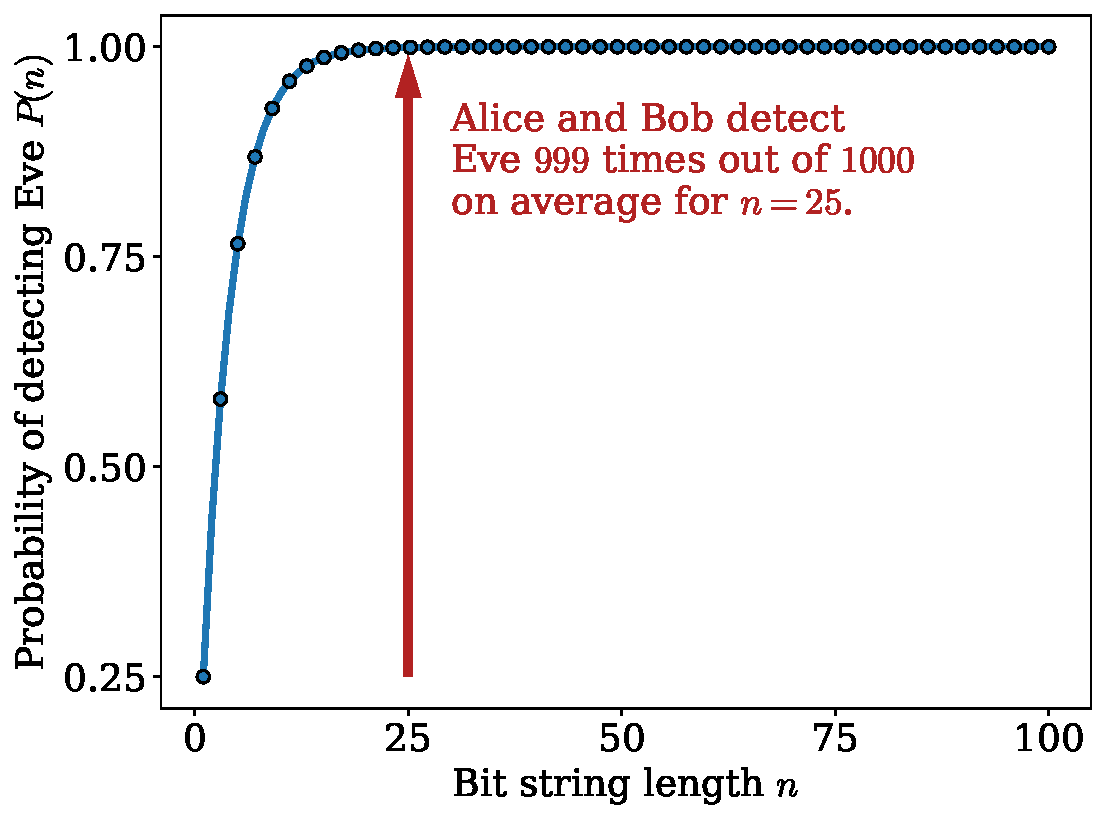
\includegraphics[width=0.8\textwidth]{lesson9/9-4_detection.pdf}
        \caption[Probability of detecting the presence of Eve]{The probability of Alice and Bob detecting the presence of Eve reaches $0.999$ with only $25$ samples.}
    \label{fig:catching-eve}
\end{figure}

In Fig.~\ref{fig:catching-eve}, on the horizontal axis, we plot $n$, the length of the bit string that we have dedicated to detecting the eavesdropper, Eve. On the vertical axis, we have the probability of detecting Eve.  When we dedicate only a few bits to actually trying to detect the eavesdropper, $n$ is very small and the probability that Eve is detected is relatively small. But very quickly, this probability shoots up very close to one. So with nearly a probability of hundred percent, Alice and Bob can detect the presence of an eavesdropper. Even for $n = 25$, dedicating a mere 25 bits to detecting Eve, the chance is only one in a thousand that Eve will not be detected.  With very high probability, Alice and Bob know that somebody's eavesdropping onto their channel, in which case they say to each other, "We know that we are not sharing a secure secret key, therefore we choose not to continue with the rest of our communication," preventing Eve from gaining access to the sensitive messages they had planned to exchange.

\section{Existing QKD network testbeds}

\rdv{Needs just a little cleanup, and to decide if we are going to try to include figures or not.}

In the previous sections, we have seen how Alice and Bob can use quantum mechanics to discover an eavesdropper and generate a secret random key for secret communication. In this step, we will demonstrate that actually these things are not only in the realm of theoretical research, but also have been tested by building real networks.

The very first network that was built was known as the DARPA QKD network, all the way back in 2004. This included ten nodes in a network, and it was built in the state of Massachusetts in the USA. It included different physical links, for example, you had a communication over free space, here you had a communication over a fiber. This was unlike any of the previous experimental implementations, where secure quantum communication in the form of a single photon-based QKD was done only on a point-to-point basis over a single link. This was the first network experiment demonstrating the viability of quantum key distribution.  This work was led by Chip Elliott of BBN, and included a version of the IPsec Internet protocol security suite adapted for QKD.  IPsec usually uses the canonical set of RSA or pre-shared secret for authentication, Diffie-Hellman for key establishment, and 3-DES or AES for bulk data encryption.  In the DARPA QKD network, the Diffie-Hellman process was replaced with keys generated by QKD.

The next experimental effort was in Europe, known as the SECOQC QKD network. SECOQC stands for "Secure Communication based on Quantum Cryptography", around the year 2008. It launched in Vienna, and it comprised six nodes and eight links. This project developed a layered architecture for the communication services. And finally, there are many other experiments but one notable one was done in Tokyo around 2010, known as the Tokyo QKD network. The University of Tokyo Hongo campus and a facility in Otemachi, a place in central Tokyo where many telecommunication providers converge, are only a few kilometers apart.  The network reached all the way to the National Institute of Information and Communications Technology (NICT) in Kogane, in the western Tokyo suburbs. The interesting part about this network is that actually it was used for a quantum secure video conference, which really demonstrated the viability of using quantum mechanics for securing communication in a network.

\rdv{China?}

\newpage
\begin{exercises}
\exer{Prove that an eavesdropper can retrieve at least some information if Alice reuses the one-time pad key bits $c$ to encrypt two separate messages $m$ and $m'$.}

\exer{In Sec.~\ref{sec:bb84-protocol}, we asserted that \ket{0} and \ket{+} are not orthogonal, and made statements about measurement probabilities without working through the mathematics.\
\subexer{Prove that the states are not orthogonal.}
\subexer{Find the probability of the $\pm 1$ outcomes when measuring both of those states in the $Z$ basis, using calculations similar to those in Sec.~\ref{sec:measurement}.}
\subexer{Find the probability of the $\pm 1$ outcomes when measuring both of those states in the $X$ basis, using calculations similar to those in Sec.~\ref{sec:measurement}.}
}


\end{exercises}

